\subsection{Epidemiologia}


HAV è presente in tutto il mondo, particolarmente in Paesi in condizioni
igienico sanitarie scadenti, tanto che l'incidenza di HAV è un
indicatore delle condizioni di sviluppo.

La forma silente può essere cercata con la ricerca degli anticorpi nella
popolazione:

\begin{itemize}
\item
  98\% in India
\item
  10\% in USA
\item
  5\% in Svizzera
\end{itemize}

\emph{Secondo l'OMS la prevalenza è di circa 1,5 milioni di casi clinici
(sintomatici) ogni anno, nel mondo.}

Dal punto di vista dell'andamento dell'infezione, questo è generalmente
sporadica, ma vi possono essere epidemie nelle comunità a rischio, come
quelle infantili o i collegi, per le condizioni igieniche più favorevoli
alla diffusione, l'affollamento, le abitudini alimentari. Gli ultimi
dati europei vedono un trend in salita della malattia e la distribuzione
per età vede come massimo peso i bambini e gli anziani.

Riassumendo i fattori di rischio sono:

\begin{itemize}
\item
  persone a contatto con soggetti infetti
\item
  bambini in comunità chiuse
\item
  viaggiatori in aree endemiche
\item
  tossicodipendenti
\end{itemize}

NB: Ci sono zone ad alta, moderata, bassa e molto bassa endemia, legate
alla prevalenza dei diversi fattori di rischio (per esempio nelle zone a
molto bassa endemia, la presenza di questo virus è essenzialmente legata
ai viaggiatori).

\subsubsection{Epidemiologia in Italia}


\begin{itemize}
\item
  La siero-epidemiologia della popolazione italiana vede una
  distribuzione del virus con prevalenza al sud, con incremento della
  positività agli anticorpi con il crescere dell'età: dopo i 40 anni più
  del 50\% della popolazione ha gli anticorpi (senza storia di malattia
  evidente).
\item
  Importanti nella nostra realtà epidemiologica sono i viaggiatori: si
  stima che la prevalenza sia da 30 a 300 casi per 10.000 viaggiatori in
  un mese di viaggio.
\item
  La principale sorgente di infezione è il portatore sano, così come il
  portatore precoce. Non abbiamo mai il portatore cronico.
\item
  La principale \emph{età} nella quale si va incontro all'infezione è
  quella giovanile: 15-24 anni
\item
  Tra tutte le epatiti, HAV prevale in assoluto, con forti epidemie nel
  1997 e nel 2007, ma anche piccoli e medi focolai epidemici nel 2001,
  2004, 2009 e 2013, collocati principalmente al sud.
\end{itemize}

\begin{figure}[!ht]
\centering
	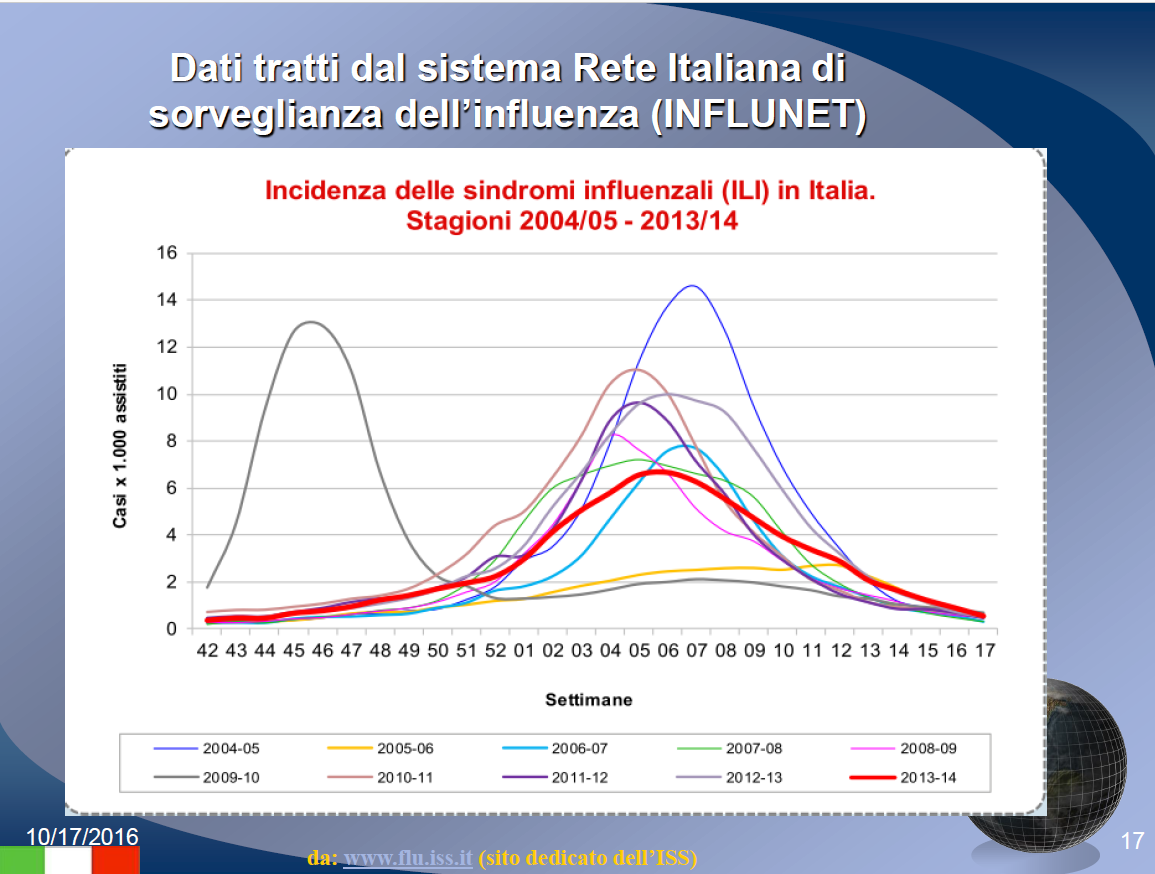
\includegraphics[width=0.7\textwidth]{02/image3.png}
\end{figure}


\begin{itemize}
\item
  FATTORI DI RISCHIO DOCUMENTATI IN ITALIA:

  \begin{itemize}
  \item
    Viaggio all'estero (è il più importante)
  \item
    Per l'alimentazione: il consumo di militii, soprattutto in certe
    regioni e in certi periodi dell'anno
  \item
    Contatti di familiari infetti
  \end{itemize}
\end{itemize}
\subsection{Prevenzione}


\begin{enumerate}
\def\labelenumi{\arabic{enumi}.}
\item
  INDIRETTA: è un aspetto di tipo generale, ha una valenza molteplice e
  in questo caso vale per TUTTI gli agenti del circuito fecale-orale, in
  linea di massima. È rivolta sia all'ambiente che alla persona.

  \begin{enumerate}
  \def\labelenumii{\alph{enumii}.}
  \item
    CONTROLLO DELLA MATRICE AMBIENTALE

    \begin{enumerate}
    \def\labelenumiii{\roman{enumiii}.}
    \item
      Alimenti: controllo della produzione e vendita, soprattutto dei
      frutti di mare, che assumono nutrienti attraverso la filtrazione
      dell'acqua in cui vivono, perciò la concentrazione dei patogeni
      all'interno di questi è molto più concentrata (in termini
      logaritmici) rispetto alle acque in cui si trovano.
    \item
      Acqua: controllo di acqua, perché sia igienicamente sicura, e
      offrire a tutta la popolazione l'acqua potabile
    \item
      Controllo del trattamento e dello smaltimento dei liquami fognari
    \item
      Lotta ai vettori (mosche) con disinfestazione
    \end{enumerate}
  \item
    EDUCAZIONE SANITARIA (in realtà è una via di mezzo tra prevenzione
    indiretta e diretta): consiste nell'importanza del rispetto delle
    norme igieniche per coloro che:

    \begin{enumerate}
    \def\labelenumiii{\roman{enumiii}.}
    \item
      Manipolano o servono alimenti
    \item
      Sono addetti all'assistenza di bambini o di malati
    \end{enumerate}
  \end{enumerate}
\item
  DIRETTA: mirata al virus


\begin{itemize}
\item
   
  \emph{Denuncia Obbligatoria} {[}Classe II{]}
   
\item
   
  \emph{Isolamento:} non obbligatorio, ma importante dal punto di vista
  dell'igiene, per contenere l'infezione nell'ambiente del malato
   
\item
   
  \emph{Inchiesta epidemiologica,} per capire perché si sia manifestata
  la patologia ed individuare la sorgente e il veicolo di infezione
   
\item
   
  \emph{Disinfezione continua e terminale} (il virus è discretamente
  resistente in ambiente e in acqua)
   
\item
   
  \emph{Profilassi Immunitaria Specifica:} esiste un vaccino per HAV.
   
\end{itemize}
\end{enumerate}
\subsubsection{Immunoprofilassi attiva: il Vaccino per HAV}


Il vaccino è stato ottenuto con virus ucciso, coltivato su cellule
diploidi umane e inattivato con formolo, da somministrare per via
intramuscolare profonda (come tutti i vaccini con patogeni inattivati).
Le dosi per una completa vaccinazione sono a 0-1-6 mesi e l'efficacia è
molto elevata: nel 90\% dei vaccinati è documentabile la presenza di IgG
dopo la prima dose e la totalità nella seconda dose con anticorpi
duraturi. La terza dose ha proprio la funzione di aumentare in titolo
anticorpale e l'efficacia del vaccino nel tempo che si attesta intorno
ai 20 anni.
\\\\
\emph{Effetti collaterali del vaccino:} dolorabilità, cefalea e
malessere di breve durata.

\paragraph{Strategia vaccinale}


\begin{itemize}
\item
  \emph{Pre-esposizione:} è consigliato il vaccino:

  \begin{itemize}
  \item
    In primis ai viaggiatori in aree endemiche, almeno due dosi o dosi
    doppie se il tempo prima del viaggio è breve
  \item
    Ai soggetti che vivono in zone ad alta endemia
  \item
    A soggetti che sono a rischio di contatto in ambito lavorativo
    (operatori sanitari e addetti allo smaltimento dei rifiuti)
  \item
    Ai militari che prestano servizio in aree endemiche
  \item
    Soggetti con handicap istituzionalizzati (per incapacità fisica o
    mentale di mettere in atto le norme igieniche)
  \item
    Soggetti con malattie croniche
  \item
    Tossicodipendenti
  \end{itemize}
\item
  \emph{Post-esposizione:} c'è la possibilità di applicare il vaccino
  post-esposizione: anche se oggi non si hanno ancora dati scientifici
  certi, data l'elevata quantità di anticorpi prodotti dopo una sola
  somministrazione, si può utilizzare questa modalità in un focolaio
  epidemico, proprio all'inizio dell'epidemia, per contenere il
  contagio.
\end{itemize}

\subsubsection{Immunoprofilassi Passiva}



In caso di probabile contagio è possibile usare le immunoglobuline
specifiche, che potrebbero essere previste anche come somministrazione
pre esposizione per i viaggiatori in aree a media ed alta endemia, e
soprattutto post esposizione per contatti a rischio.


\section{Epatite E (HEV)}



\subsection{Caratteristiche e Cenni clinici }


Il virus dell'epatite E è stato scoperto in un focolaio endemico in
India. È trasmesso attraverso un circuito fecale-orale e ha periodo di
incubazione simile all'HAV, di circa 40 giorni (range dai 15 ai 60
giorni).

Ha una notevole importanza nelle donne in gravidanza dove l'infezione si
associa ad una letalità del 15-25\% dei casi, contro la letalità nella
popolazione generale dell'1-3\%. La gravità della malattia aumenta con
il crescere dell'età, ma il virus NON determina MAI CRONICIZZAZIONE.

\emph{La diagnosi si avvale di:}

\begin{itemize}
\item
  Clinica
\item
  Anticorpi specifici
\item
  Ricerca di acidi nucleici (attraverso RT-PCR) in campioni di sangue e
  feci
\end{itemize}

\subsection{Epidemiologia e Profilassi}


\emph{La distribuzione del mondo}: HEV è prevalente nel subcontinente
indiano, dove è stato identificato, ed è più presente in Paesi in via di
sviluppo che nei Paesi industrializzati. Secondo la WHO nel 2014 si sono
registrati circa \emph{20 milioni di casi a livello mondiale.}

Si sono verificati dei focolai epidemici, quasi sempre associati
all'acqua contaminata da liquami fognari; è rarissimo il contagio
interumano. Negli USA, dove ci sono più dati, l'infezione da HEV è
generalmente associata a viaggi in zone endemiche. In \emph{Italia} è
rara, ma si sono registrati negli ultimi anni dei focolai epidemici
nelle regioni centrali.
\subsection{Prevenzione}


Si possono solo attuare solamente delle azioni di \emph{prevenzione
generale} per coloro che si recano in Paesi endemici, per esempio:

\begin{itemize}
\item
  Utilizzare sempre e solo acqua potabile (in contenitori tappati)
\item
  Non bere bibite con ghiaccio
\item
  Consumare frutti di mare cotti (la cottura abbatte il virus)
\item
  Consumare verdure preferibilmente cotte e la frutta è da sbucciare
  dopo il lavaggio
\end{itemize}

Non abbiamo dati su eventuale immunoprofilassi con IgG e non abbiamo un
vaccino globalmente accettato, anche se nel 2011 in Cina è stato
licenziato un vaccino specifico.
\section{Febbre Tifoide}

\subsection{Caratteristiche e Cenni clinici}


Malattia infettiva determinata da Salmonella Typhi, che appartiene alla
famiglia delle salmonelle ed è dotata di alcuni \emph{antigeni:}

\begin{itemize}
\item
  Antigene O: somatico
\item
  Antigene H: flagellare
\item
  Antigene Vi: capsulare
\end{itemize}

Ed è proprio verso questi antigeni che vengono prodotti gli anticorpi
protettivi, il più importante è quello verso l'antigene capsulare,
l'anticorpo anti-Vi, insieme anche all'anti-O.

La febbre tifoide è una malattia molto meno frequente che nel passato;
al giorno d'oggi, in assenza di terapia, presenta una letalità che va
dall'1 al 10\% a seconda delle aree.

Il problema attuale è la crescente farmaco resistenza, molto più
presente nei Paesi del terzo mondo, in particolare in alcune regioni del
sud est asiatico (dove si calcola che il 70\% dei ceppi isolati presenta
una farmaco resistenza).

\subsection{Storia naturale della malattia }

Trasmesso per via fecale orale, è in grado di superare la barriera
gastrica e ciò avviene più facilmente se:

\begin{itemize}
\item
  è presente in carica virale molto elevata
\item
  si consuma un pasto ricco di proteine (che hanno un'azione
  neutralizzante l'acidità gastrica)
\item
  si beve acqua in quantità abbondante (diluizione)
\item
  si ha una condizione di ipocloridia gastrica
\end{itemize}

da qui, dopo una prima fase di replicazione (in era pre antibiotica) il
batterio passa alle strutture linfatiche della parete intestinale -> dotto
toracico -> diffusione ematica -> diffusione ai linfonodi -> dal fegato
attraverso la bile torna una seconda volta a livello intestinale, dove
si realizza la seconda replicazione, con la moltiplicazione in strutture
già sensibilizzate: questo innesca un grosso processo flogistico con
escare e necrosi, ulcerazioni, fino ad avere lesioni vascolari,
emorragie e quindi la morte del paziente.

L'accertamento diagnostico permette di individuare:

\begin{itemize}
\item
  nella prima settimana, la presenza del patogeno nel sangue, attraverso
  emocoltura
\item
  nella seconda settimana anticorpi anti-O e anti-H con
  sieroagglutinazione
\item
  nella terza e quarta settimana la ricerca del patogeno nella
  coprocoltura. Il patogeno può essere abbondantemente presente anche
  nelle urine.
\end{itemize}

\subsection{Epidemiologia e Profilassi}


L'infezione si registra prevalentemente nei Paesi sottosviluppati,
Indonesia, Guinea, Haiti, che oltre ad essere paesi dal clima caldo
presentano condizioni igienico-sanitarie scadenti.

\emph{In Europa} la prevalenza è calata notevolmente nell'ultimo
decennio, ma rimane ancora discreta la prevalenza negli stati dell'est.

\emph{In Italia} l'incidenza si attesta intorno a 1/100.000 casi
all'anno, con prevalenza maggiore al sud e nelle isole, dove abitudini
alimentari, condizioni igieniche, ma anche cultura alimentare (consumo
di frutti di mare crudi) favoriscono la diffusione della malattia.

\subsection{Sorgente d'infezione}


È un'infezione esclusivamente umana (diversamente dalle altre
salmonelle) e le principali sorgenti di infezione sono il malato, ma
anche il portatore convalescente e il portatore cronico.

La \emph{trasmissione è per via fecale orale}: possiamo rifarci a ciò
che era stato detto a riguardo nel HAV.

Si noti che nel nord-Italia si registrano dei casi nel periodo post
Natale in soggetti che durante le vacanze si recano nei paesi di
origine, acquisiscono le abitudini alimentari, tornano in Italia e
manifestano la malattia. È un'infezione molto più frequente nel bambino
e nel giovane adulto.

\subsection{Prevenzione}


Per la \emph{profilassi indiretta}: vale esattamente il discorso fatto
per HAV, con il controllo delle matrici ambientali e l'educazione alla
salute (che valgono per tutte le patologie del circuito fecale-orale).
\\\\
La \emph{profilassi diretta}:

\begin{itemize}
\item
   
  \emph{Denuncia Obbligatoria} {[}Classe II{]}
   
\item
   
  \emph{Isolamento:} non obbligatorio, ma è importante dal punto di
  vista dell'igiene, per contenere l'infezione nell'ambiente del malato.
  Tre campioni di feci devono risultare negativi dopo l'inizio del
  trattamento antibiotico per considerare il soggetto non più
  infettante.
   
\item
   
  \emph{Accertamento diagnostico:} importante perché c'è la figura del
  portatore cronico
   
\item
   
  \emph{Inchiesta epidemiologica,} per capire perché si sia manifestata
  la patologia ed individuare la sorgente e il veicolo di infezione
   
\item
   
  \emph{Disinfezione continua} (le feci sono contaminate per lungo
  tempo) \emph{e terminale e disinfestazione} (mosche)
   
\item
   
  \emph{Profilassi Immunitaria Specifica:} esiste un vaccino specifico
  per S. typhi.
   
\end{itemize}

\subsubsection{Immunoprofilassi Attiva}


È stata una delle patologie più studiate e quello verso la Salmomella
Typhi è stato il vaccino più precocemente ricercato nella storia, tanto
che sono state tentate tantissime strade per la sua realizzazione.

Ad oggi disponiamo di 3 vaccini:

\begin{itemize}
\item
  Il vecchio vaccino, ancora utilizzato, somministrato per via
  parenterale
\item
  Vaccino Ty21: vivo ed attenuato ad uso naturale, viene somministrato
  per via orale segue la via dell'infezione naturale.

  \begin{itemize}
  \item
    È stato ottenuto privando il batterio virulento di un enzima, che
    rende il batterio incapace di incorporare galattosio nel LPS della
    parete cellulare. Il ceppo si sviluppa come variante rugosa non
    patogena, inizialmente non immunizzante, ma quando giunge in un
    ambiente ricco di galattosio (come l'intestino), questo zucchero
    viene assunto dall'ambiente, utilizzato per la costruzione della
    parete cellulare e il patogeno riesce a fare una serie di cicli
    replicativi (il batterio diventa così immunizzante), ma non riesce
    ad eliminare il galattosio accumulato, quindi esso si autolisa
    proprio per l'eccesso osmotico: questa salmonella non viene dunque
    eliminata con le feci e il patogeno è divenuto sì immunizzante
    nell'intestino, ma non esce come virulento, grazie al processo di
    autolisi: perciò non è diffuso nell'ambiente
  \item
    È molto immunizzante (efficacia maggiore dell'87\% per più di 3
    anni)
  \item
    Viene assunto in capsule gastroresistenti un'ora prima del pasto per
    3 giorni, a giorni alterni, e si può ripetere per mantenere
    l'immunità elevata per tempi lunghi
  \item
    Non abbiamo dati per un'eventuale utilizzo post esposizione del
    vaccino
  \item
    NB: essendo un vaccino con ceppo vivo non possiamo somministrarlo in
    concomitanza con la terapia antibiotica
  \end{itemize}
\item
  \emph{Vaccino a componente Vi:} somministrato per via parenterale, ha
  efficacia circa uguale al vaccino Ty21, con durata di circa 3 anni. È
  ben tollerabile.
\end{itemize}

\paragraph{Indicazioni per la vaccinazione:}


\begin{itemize}
\item
  In primis c'è una forte indicazione (ma non l'obbligo) per chi si reca
  in aree endemiche
\item
  A chi svolge attività a rischio, come pulizia di ospedali, personale
  addetto al trasporto di malati
\item
  Agli operatori sanitari
\item
  Al personale addetto all'approvvigionamento idrico e alla
  manipolazione del latte
\item
  Al personale addetto alla raccolta e allo smaltimento dei rifiuti
\item
  A chi svolge manipolazione e vendita di alimenti: in passato il
  vaccino era d'obbligo (DPR n 327/1980), ma oggi l'igiene degli
  ambienti è regolata dalle regioni, che hanno sostituito il libretto
  sanitario con controlli degli ambienti e corsi di formazione tenuti
  dalle AUSL
\end{itemize}

